% RTAS Demo Abstract
%

%% bare_conf.tex
%% V1.3
%% 2007/01/11
%% by Michael Shell
%% See:
%% http://www.michaelshell.org/
%% for current contact information.
%%
%% This is a skeleton file demonstrating the use of IEEEtran.cls
%% (requires IEEEtran.cls version 1.7 or later) with an IEEE conference paper.
%%
%% Support sites:
%% http://www.michaelshell.org/tex/ieeetran/
%% http://www.ctan.org/tex-archive/macros/latex/contrib/IEEEtran/
%% and
%% http://www.ieee.org/

%%*************************************************************************
%% Legal Notice:
%% This code is offered as-is without any warranty either expressed or
%% implied; without even the implied warranty of MERCHANTABILITY or
%% FITNESS FOR A PARTICULAR PURPOSE! 
%% User assumes all risk.
%% In no event shall IEEE or any contributor to this code be liable for
%% any damages or losses, including, but not limited to, incidental,
%% consequential, or any other damages, resulting from the use or misuse
%% of any information contained here.
%%
%% All comments are the opinions of their respective authors and are not
%% necessarily endorsed by the IEEE.
%%
%% This work is distributed under the LaTeX Project Public License (LPPL)
%% ( http://www.latex-project.org/ ) version 1.3, and may be freely used,
%% distributed and modified. A copy of the LPPL, version 1.3, is included
%% in the base LaTeX documentation of all distributions of LaTeX released
%% 2003/12/01 or later.
%% Retain all contribution notices and credits.
%% ** Modified files should be clearly indicated as such, including  **
%% ** renaming them and changing author support contact information. **
%%
%% File list of work: IEEEtran.cls, IEEEtran_HOWTO.pdf, bare_adv.tex,
%%                    bare_conf.tex, bare_jrnl.tex, bare_jrnl_compsoc.tex
%%*************************************************************************

% *** Authors should verify (and, if needed, correct) their LaTeX system  ***
% *** with the testflow diagnostic prior to trusting their LaTeX platform ***
% *** with production work. IEEE's font choices can trigger bugs that do  ***
% *** not appear when using other class files.                            ***
% The testflow support page is at:
% http://www.michaelshell.org/tex/testflow/



% Note that the a4paper option is mainly intended so that authors in
% countries using A4 can easily print to A4 and see how their papers will
% look in print - the typesetting of the document will not typically be
% affected with changes in paper size (but the bottom and side margins will).
% Use the testflow package mentioned above to verify correct handling of
% both paper sizes by the user's LaTeX system.
%
% Also note that the "draftcls" or "draftclsnofoot", not "draft", option
% should be used if it is desired that the figures are to be displayed in
% draft mode.
%
\documentclass[conference]{IEEEtran}
% Add the compsoc option for Computer Society conferences.
%
% If IEEEtran.cls has not been installed into the LaTeX system files,
% manually specify the path to it like:
% \documentclass[conference]{../sty/IEEEtran}





% Some very useful LaTeX packages include:
% (uncomment the ones you want to load)


% *** MISC UTILITY PACKAGES ***
%

% *** CITATION PACKAGES ***
%
\usepackage{cite}
% cite.sty was written by Donald Arseneau
% V1.6 and later of IEEEtran pre-defines the format of the cite.sty package
% \cite{} output to follow that of IEEE. Loading the cite package will
% result in citation numbers being automatically sorted and properly
% "compressed/ranged". e.g., [1], [9], [2], [7], [5], [6] without using
% cite.sty will become [1], [2], [5]--[7], [9] using cite.sty. cite.sty's
% \cite will automatically add leading space, if needed. Use cite.sty's
% noadjust option (cite.sty V3.8 and later) if you want to turn this off.
% cite.sty is already installed on most LaTeX systems. Be sure and use
% version 4.0 (2003-05-27) and later if using hyperref.sty. cite.sty does
% not currently provide for hyperlinked citations.
% The latest version can be obtained at:
% http://www.ctan.org/tex-archive/macros/latex/contrib/cite/
% The documentation is contained in the cite.sty file itself.

% *** GRAPHICS RELATED PACKAGES ***
%
\usepackage[pdftex]{graphicx}
% declare the path(s) where your graphic files are
\graphicspath{{./figures/}}
% and their extensions so you won't have to specify these with
% every instance of \includegraphics
\DeclareGraphicsExtensions{.pdf,.jpeg,.png}

% graphicx was written by David Carlisle and Sebastian Rahtz. It is
% required if you want graphics, photos, etc. graphicx.sty is already
% installed on most LaTeX systems. The latest version and documentation can
% be obtained at: 
% http://www.ctan.org/tex-archive/macros/latex/required/graphics/
% Another good source of documentation is "Using Imported Graphics in
% LaTeX2e" by Keith Reckdahl which can be found as epslatex.ps or
% epslatex.pdf at: http://www.ctan.org/tex-archive/info/
%
% latex, and pdflatex in dvi mode, support graphics in encapsulated
% postscript (.eps) format. pdflatex in pdf mode supports graphics
% in .pdf, .jpeg, .png and .mps (metapost) formats. Users should ensure
% that all non-photo figures use a vector format (.eps, .pdf, .mps) and
% not a bitmapped formats (.jpeg, .png). IEEE frowns on bitmapped formats
% which can result in "jaggedy"/blurry rendering of lines and letters as
% well as large increases in file sizes.
%
% You can find documentation about the pdfTeX application at:
% http://www.tug.org/applications/pdftex

% *** MATH PACKAGES ***
%
\usepackage[cmex10]{amsmath}
% A popular package from the American Mathematical Society that provides
% many useful and powerful commands for dealing with mathematics. If using
% it, be sure to load this package with the cmex10 option to ensure that
% only type 1 fonts will utilized at all point sizes. Without this option,
% it is possible that some math symbols, particularly those within
% footnotes, will be rendered in bitmap form which will result in a
% document that can not be IEEE Xplore compliant!
%
% Also, note that the amsmath package sets \interdisplaylinepenalty to 10000
% thus preventing page breaks from occurring within multiline equations. Use:
%\interdisplaylinepenalty=2500
% after loading amsmath to restore such page breaks as IEEEtran.cls normally
% does. amsmath.sty is already installed on most LaTeX systems. The latest
% version and documentation can be obtained at:
% http://www.ctan.org/tex-archive/macros/latex/required/amslatex/math/

% *** SPECIALIZED LIST PACKAGES ***
%
%\usepackage{algorithmic}
% algorithmic.sty was written by Peter Williams and Rogerio Brito.
% This package provides an algorithmic environment fo describing algorithms.
% You can use the algorithmic environment in-text or within a figure
% environment to provide for a floating algorithm. Do NOT use the algorithm
% floating environment provided by algorithm.sty (by the same authors) or
% algorithm2e.sty (by Christophe Fiorio) as IEEE does not use dedicated
% algorithm float types and packages that provide these will not provide
% correct IEEE style captions. The latest version and documentation of
% algorithmic.sty can be obtained at:
% http://www.ctan.org/tex-archive/macros/latex/contrib/algorithms/
% There is also a support site at:
% http://algorithms.berlios.de/index.html
% Also of interest may be the (relatively newer and more customizable)
% algorithmicx.sty package by Szasz Janos:
% http://www.ctan.org/tex-archive/macros/latex/contrib/algorithmicx/

% *** ALIGNMENT PACKAGES ***
%
%\usepackage{array}
% Frank Mittelbach's and David Carlisle's array.sty patches and improves
% the standard LaTeX2e array and tabular environments to provide better
% appearance and additional user controls. As the default LaTeX2e table
% generation code is lacking to the point of almost being broken with
% respect to the quality of the end results, all users are strongly
% advised to use an enhanced (at the very least that provided by array.sty)
% set of table tools. array.sty is already installed on most systems. The
% latest version and documentation can be obtained at:
% http://www.ctan.org/tex-archive/macros/latex/required/tools/


%\usepackage{mdwmath}
%\usepackage{mdwtab}
% Also highly recommended is Mark Wooding's extremely powerful MDW tools,
% especially mdwmath.sty and mdwtab.sty which are used to format equations
% and tables, respectively. The MDWtools set is already installed on most
% LaTeX systems. The lastest version and documentation is available at:
% http://www.ctan.org/tex-archive/macros/latex/contrib/mdwtools/


% IEEEtran contains the IEEEeqnarray family of commands that can be used to
% generate multiline equations as well as matrices, tables, etc., of high
% quality.


%\usepackage{eqparbox}
% Also of notable interest is Scott Pakin's eqparbox package for creating
% (automatically sized) equal width boxes - aka "natural width parboxes".
% Available at:
% http://www.ctan.org/tex-archive/macros/latex/contrib/eqparbox/








% *** FLOAT PACKAGES ***
%
%\usepackage{fixltx2e}
% fixltx2e, the successor to the earlier fix2col.sty, was written by
% Frank Mittelbach and David Carlisle. This package corrects a few problems
% in the LaTeX2e kernel, the most notable of which is that in current
% LaTeX2e releases, the ordering of single and double column floats is not
% guaranteed to be preserved. Thus, an unpatched LaTeX2e can allow a
% single column figure to be placed prior to an earlier double column
% figure. The latest version and documentation can be found at:
% http://www.ctan.org/tex-archive/macros/latex/base/



%\usepackage{stfloats}
% stfloats.sty was written by Sigitas Tolusis. This package gives LaTeX2e
% the ability to do double column floats at the bottom of the page as well
% as the top. (e.g., "\begin{figure*}[!b]" is not normally possible in
% LaTeX2e). It also provides a command:
%\fnbelowfloat
% to enable the placement of footnotes below bottom floats (the standard
% LaTeX2e kernel puts them above bottom floats). This is an invasive package
% which rewrites many portions of the LaTeX2e float routines. It may not work
% with other packages that modify the LaTeX2e float routines. The latest
% version and documentation can be obtained at:
% http://www.ctan.org/tex-archive/macros/latex/contrib/sttools/
% Documentation is contained in the stfloats.sty comments as well as in the
% presfull.pdf file. Do not use the stfloats baselinefloat ability as IEEE
% does not allow \baselineskip to stretch. Authors submitting work to the
% IEEE should note that IEEE rarely uses double column equations and
% that authors should try to avoid such use. Do not be tempted to use the
% cuted.sty or midfloat.sty packages (also by Sigitas Tolusis) as IEEE does
% not format its papers in such ways.





% *** PDF, URL AND HYPERLINK PACKAGES ***
%
%\usepackage{url}
% url.sty was written by Donald Arseneau. It provides better support for
% handling and breaking URLs. url.sty is already installed on most LaTeX
% systems. The latest version can be obtained at:
% http://www.ctan.org/tex-archive/macros/latex/contrib/misc/
% Read the url.sty source comments for usage information. Basically,
% \url{my_url_here}.





% *** Do not adjust lengths that control margins, column widths, etc. ***
% *** Do not use packages that alter fonts (such as pslatex).         ***
% There should be no need to do such things with IEEEtran.cls V1.6 and later.
% (Unless specifically asked to do so by the journal or conference you plan
% to submit to, of course. )


% correct bad hyphenation here
\hyphenation{op-tical net-works semi-conduc-tor}





\begin{document}

\title{Demo Abstract: The ESMoL Modeling Language and Tools for Synthesizing and Simulating Real-Time Embedded Systems}

\author{\IEEEauthorblockN{Joseph Porter, Zsolt Lattmann, Graham Hemingway,   
Nagabhushan Mahadevan, Sandeep Neema, \\
Harmon Nine, Nicholas Kottenstette, P\'{e}ter V\"{o}lgyesi, G\'{a}bor Karsai, and J\'{a}nos Sztipanovits}
\IEEEauthorblockA{Institute for Software Integrated Systems \\
Vanderbilt University\\
Nashville, TN 37235, USA \\
Email: jporter@isis.vanderbilt.edu\\
Telephone: (615) 343--4641}
}

\maketitle

\begin{abstract}
High-confidence embedded real-time designs stretch the demands placed
on design and development tools.  We will demonstrate the design and
testing of an embedded control system built using the ESMoL modeling
language and supporting tools.  ESMoL adds distributed deployment 
concepts to Simulink designs, and integrates scheduling analysis as well
as platform-specific simulation.  The testing system includes a simulated
physical plant running in a hardware-in-the-loop configuration with the
actual embedded controller.
\end{abstract}

\section{Introduction}

Many classes of real-time embedded systems require assurance that 
engineering designs and implementations are safe, secure, and correct.  
Examples include software for medical devices, weapons control systems, 
and aircraft flight control.  The time and effort (and consequently cost)
of such assurance stands in contrast with the cost and schedule pressures
of production engineering.

The ESMoL (Embedded Systems Modeling Language) domain-specific modeling 
language (DSML) provides user modeling constructs for designing 
embedded systems -- including functional specifications in Simulink, 
models for distributed computing platforms, and deployment models assigning 
functions to tasks on computing nodes\cite{aces08}.  The language structure 
and the supporting Model-Integrated Computing (MIC) tools \cite{mic:metaprog} 
enable the integration of analysis tools to provide design assurance for use 
in high-confidence designs.

\begin{figure}[!b]
\centering
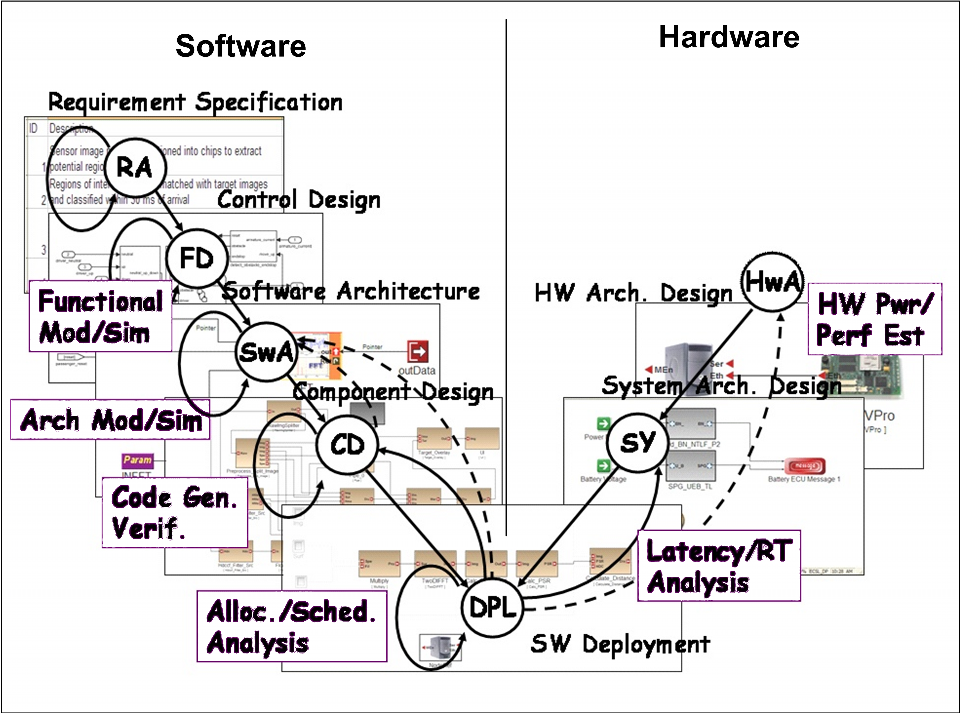
\includegraphics[width=0.9\columnwidth]{vdiagram}
\caption{Embedded development workflow supported by the tools.}
\label{fig:vdiagram}
\end{figure}

The development workflow supported by the tools is depicted in 
Fig. \ref{fig:vdiagram}.  After the Requirements Specification 
has been created, designers start with familiar tools like Simulink to
design and simulate the functional control system (Control Design).  
The Simulink design is imported into the modeling 
environment, and then annotated with Software Architecture and Component 
Design concepts.  Platform models (Hardware and System Architecture 
Design) represent the hardware architecture.  Componentized functions 
and signals are then assigned to tasks and messages deployed on the 
hardware (Software Deployment). From the composed model we can perform 
static real-time schedule determination and synthesize code for a distributed 
platform -- assuming the platform provides clocked synchronous task execution 
and time-triggered messaging services.  

The tools currently support development for unmanned aerial vehicles,
in particular the Starmac quadrotor helicopter \cite{HRWDJT04}.  The control
architecture is based on a fast inner-loop controller for attitude (here simplified
to angle) and a slower outer-loop controller for position (here simplified to a
scalar value).  Our control technique is based on a composition of nested passive 
(PD) controllers to stabilize a process modeled as a cascade of continuous-time 
systems \cite[Fig.~1]{kottenstette08:_digit_passiv_attit_and_altit}.  

\section{Tool Features and Progress}

The enabling ideas (beyond the existing capabilities of model-based 
development) are the integration of analysis and simulation tools to 
provide meaningful feedback to designers as early as possible in the 
development cycle, and a search for decoupling techniques which help 
make required analyses tractible.  This demonstration will focus on 
the first aspect of our work (integrated analysis and simulation early in the
design cycle) for embedded software synthesized from models.  A detailed presentation 
of the design philosophy, intended uses and features, and limitations 
of the language and its tools is available in \cite{aces08}.  A few 
features are noteworthy:

\begin{enumerate}
\item   The TrueTime
toolkit \cite{TrueTime} extends Simulink with blocks for modeling 
distributed platforms to simulate uncertainties due to distributed processing. 
Our modeling tools allow resimulation of the design using TrueTime
blocks synthesized from the deployment model.  A single design model targets both the 
continuous-time platform simulation environment of TrueTime and the tasks in the 
actual distributed system.  Platform-specific simulation exposes potentially
destabilizing effects of communication delays before physical system construction.
\item Platform communication delays are captured explicitly in the models.
An integrated scheduling tool uses these timing parameters for analysis.  
Computed schedules are fed back into the modeling environment for  
TrueTime simulations and for the final physical deployment.  Designers can 
iterate over possible component and plaform design alternatives and check 
schedulability.
\item In contrast to code generation tools like Real-Time workshop
\cite{mathworks:tools} -- which generate code for individual processing 
nodes -- ESMoL generates the task configuration code as well 
as the communication glue code for the
distributed platforms on which it runs.  The network may be
a heterogeneous collection of processors and buses, as long as processing
node and communication link types are supported by the code generators.
\item The entire tool infrastructure has been built around a
single abstract semantic model, greatly simplifying the process of 
integrating additional analysis and synthesis tools.  This ensures
that all integrated tools have a single, consistent view of the 
modeling language semantics.
\end{enumerate}

Current development includes extension of the TrueTime simulation generator, 
investigations into automated quantization of the digital controllers 
(subject to safety constraints), and consideration of other tools for verification 
of control properties and deadlocks.  In particular, integration of new
tools will require expansion of the language to include
specification of richer operational models.

\section{Tool Demonstration}

The demonstration will display the following aspects the ESMoL modeling 
language and tools:

\begin{enumerate}
\item Synthesis of a Simulink control design from the GME modeling 
environment \cite{mic:gme} to run on a simple distributed embedded processing
system (Gumstix processor with an attached Robostix I/O processor
\cite{gumstix}).
\item Computation of a cyclic real-time schedule using the integrated 
Gecode constraint solver\cite{gecode}\cite{sw:offlinescheduling}.
\item Execution of the synthesized control functions on a portable 
time-triggered virtual machine (FRODO\cite{RT_Thesis}) running on the 
embedded hardware.
\item Simulation of the control loops using a hardware-in-the-loop 
(HIL) simulator communicating with the embedded system through a physical 
interface.  The HIL simulator is a PC running the Mathworks' xPC target
\cite{mathworks:tools}.  Fig. \ref{fig:sim_arch} shows the structure of
the simulation system.
\end{enumerate}

\begin{figure}[!t]
\centering
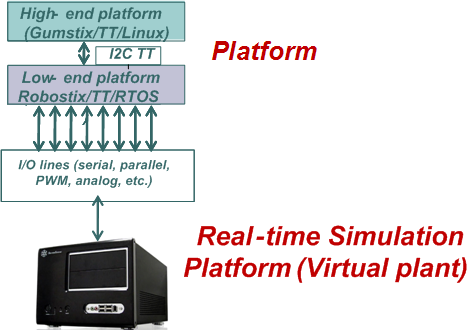
\includegraphics[width=2.5in]{sim_arch}
\caption{Hardware-in-the-loop simulation architecture. The high-end
PXA processor runs generic Linux, and the low-end AVR microcontroller runs FreeRTOS.
The two communicate via an $I^2C$ bus using a lightweight time-triggered messaging
protocol. Communication to the plant simulator PC occurs over multiple 
high-speed serial lines.}
\label{fig:sim_arch}
\end{figure}

\section*{Acknowledgment}

This work is sponsored in part by the National Science Foundation 
(grant NSF-CCF-0820088) and by the Air Force Office of Scientific 
Research, USAF (grant/contract number FA9550-06-0312).  The views 
and conclusions contained herein are those of the authors and 
should not be interpreted as necessarily representing the official 
policies or endorsements, either expressed or implied, of the Air 
Force Office of Scientific Research or the U.S. Government.

\bibliographystyle{IEEEtran}
\bibliography{rtas_demo_2009}

\end{document}
